\section{Aufgabe 3} \label{ex3}

Es wurde ein Projekt mit AXI Timer und aktiviertem Interrupt als IP Core ausgewählt. Jeder Ablauf des Timers wird 
registriert und sobald dies 3 mal eintritt, die LED Anzeige als Binärzähler um 1 inkrementiert. 
Das bedeutet, die LEDs werden in Echtzeit weitergeschaltet, da der Timer in Hardware implementiert ist und nicht abhängig 
von der CPU load oder dem Thread handling ist. Auch entfällt das polling.\\

Frei nach: https://www.youtube.com/watch?v=gaZ1kRJzCok

\begin{verbatim}
  // timer presetting & reset value
  #define TMR_LOAD  0xF8000000 // 32 bit
\end{verbatim}

Blockschaltbild in Vivado\\
\begin{minipage}{\textwidth}
    \begin{center}        
        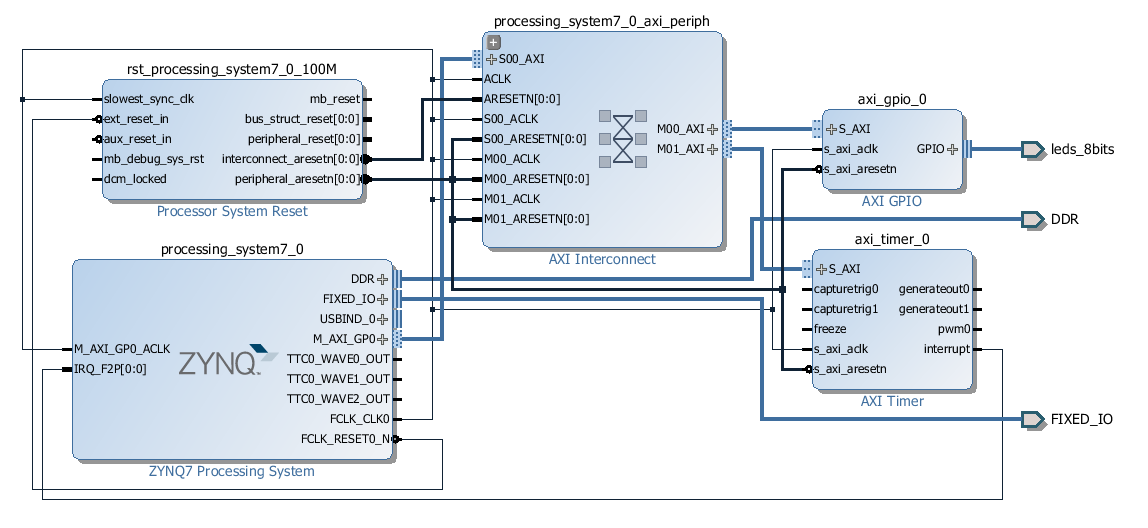
\includegraphics[scale=0.57]{img/timer3block.png} 
    \end{center}
\end{minipage}
\begin{center}
AXI Timer mit Interrupt \& AXI GPio
\end{center}


\begin{verbatim}
/*   ps7_uart    115200 (configured by bootrom/bsp) */
#include <stdio.h>
#include "platform.h"

#include "xparameters.h"
#include "xgpio.h"
#include "xtmrctr.h"
#include "xscugic.h"
#include "xil_exception.h"
#include "xil_printf.h"

// parameter definitions
#define INTC_DEVICE_ID              XPAR_PS7_SCUGIC_0_DEVICE_ID
#define TMR_DEVICE_ID               XPAR_TMRCTR_0_DEVICE_ID
#define LEDS_DEVICE_ID               XPAR_AXI_GPIO_0_DEVICE_ID
#define INTC_TMR_INTERRUPT_ID XPAR_FABRIC_AXI_TIMER_0_INTERRUPT_INTR

#define TMR_LOAD  0xF8000000
XGpio   LEDInst;
XScuGic INTCInst;
XTmrCtr TMRInst;

// only visible to module
static int led_data;
static int tmr_count;

// Prototype functions
static void TMR_Intr_Handler(void *baseeaddr_p);
static int  IntcInitFunction(u16 DeviceID, XTmrCtr *TmrInstancePtr);

void TMR_Intr_Handler(void *baseeaddr_p) {
  if (XTmrCtr_IsExpired(&TMRInst,0)) {
    // Once it has expired 3 times, stop, increment counter
    // reset timer and start running again
    if (tmr_count == 3) {
      XTmrCtr_Stop(&TMRInst,0);
      tmr_count = 0;
      led_data++;
      XGpio_DiscreteWrite(&LEDInst, 1, led_data);
      XTmrCtr_Reset(&TMRInst, 0);
      XTmrCtr_Start(&TMRInst, 0);
    } else
       tmr_count++;
  }
}

// Initial setup functions
int InterruptSystemSetup(XScuGic *XScuGicInstancePtr) {
  // Enable interrupt
  Xil_ExceptionRegisterHandler(XIL_EXCEPTION_ID_INT,
      (Xil_ExceptionHandler) XScuGic_InterruptHandler,
      XScuGicInstancePtr);
  Xil_ExceptionEnable();

  return XST_SUCCESS;
}

int  IntcInitFunction(u16 DeviceID, XTmrCtr *TmrInstancePtr) {
  XScuGic_Config *IntcConfig;
  int status;

  // Interrupt controller initialization
  IntcConfig = XScuGic_LookupConfig(DeviceID);
  status = XScuGic_CfgInitialize(&INTCInst, IntcConfig,
  IntcConfig->CpuBaseAddress);
  if (status != XST_SUCCESS)
    return XST_FAILURE;

  // Call to interrupt setup
  status = InterruptSystemSetup(&INTCInst);
  if (status != XST_SUCCESS)
    return XST_FAILURE;

  // Connect timer interrupt to handler
  status = XScuGic_Connect(&INTCInst, INTC_TMR_INTERRUPT_ID,
      (Xil_ExceptionHandler) TMR_Intr_Handler, (void *) TmrInstancePtr);
  if (status != XST_SUCCESS)
    return XST_FAILURE;

  XScuGic_Enable(&INTCInst, INTC_TMR_INTERRUPT_ID);

  return XST_SUCCESS;
}

int main()
{
  init_platform();
  print("Hello World\n\r");

  led_data = 0;
  int status;
  // ------------------------------------------------------
  // Initialize the peripherals & set directions of gpio
  // ------------------------------------------------------
  // Init LEDs
  status = XGpio_Initialize(&LEDInst, LEDS_DEVICE_ID);
  if (status != XST_SUCCESS) {
    print ("ERR: gpio failed");
    return XST_FAILURE;
  }

  // Set LEDs direction to outputs
  XGpio_SetDataDirection(&LEDInst, 1, 0x00);

  // Initialize interrupt controller
  status = IntcInitFunction(INTC_DEVICE_ID, &TMRInst);
  if (status != XST_SUCCESS) {
    print ("ERR: init interrupt controller");
    return XST_FAILURE;
  }

  // ------------------------------------------------------
  // setup the timer
  // ------------------------------------------------------
  status = XTmrCtr_Initialize(&TMRInst, TMR_DEVICE_ID);
  if (status != XST_SUCCESS) {
    print ("ERR: setup timer failed");
    return XST_FAILURE;
  }

  XTmrCtr_SetHandler(&TMRInst, (XTmrCtr_Handler) TMR_Intr_Handler, &TMRInst);
  XTmrCtr_SetResetValue(&TMRInst,0, TMR_LOAD);
  XTmrCtr_SetOptions(&TMRInst, 0,
  XTC_INT_MODE_OPTION | XTC_AUTO_RELOAD_OPTION);

  XTmrCtr_Start(&TMRInst, 0);

  printf("INFO: entering endless loop\n\r");
  while (1)
    ;

  cleanup_platform();
  return 0;
}
\end{verbatim}